\documentclass[12pt,a4paper]{article}
\usepackage[left=15mm,right=15mm,top=14mm,bottom=20mm,footskip=10mm]{geometry}
\usepackage{iftex}
\ifPDFTeX
  \usepackage[T5]{fontenc}
  \usepackage[utf8]{inputenc}
  \usepackage{mathptmx}
\else
  \usepackage{fontspec}
  \IfFontExistsTF{Times New Roman}{\setmainfont{Times New Roman}}{%
    \IfFontExistsTF{Liberation Serif}{\setmainfont{Liberation Serif}}{\setmainfont{Latin Modern Roman}}}
\fi
\usepackage{amsmath,amssymb}
\usepackage{fix-cm}
\usepackage{tikz}
\usetikzlibrary{arrows.meta}
\usepackage{tcolorbox}
\usepackage{fancyhdr}
\usepackage{lastpage}
\usepackage{tabularx}
\definecolor{sectionpurple}{RGB}{155,42,143}
\definecolor{notebackground}{RGB}{229,240,245}
\definecolor{noteborder}{RGB}{255,55,55}
\setlength{\parindent}{0pt}
\setlength{\parskip}{2pt}
\setlength{\headheight}{15pt}
\pagestyle{fancy}
\fancyhf{}
\renewcommand{\headrulewidth}{0pt}
\renewcommand{\footrulewidth}{0.4pt}
\fancyfoot[L]{\fontsize{8.5}{10}\selectfont
  Biên soạn: \textbf{Nguyễn Anh Dũng}}
\fancyfoot[R]{\fontsize{8.5}{10}\selectfont
  Trang \thepage/\pageref{LastPage} -- Đề TDMXX08}
\newtcolorbox{notebox}{colback=notebackground,colframe=noteborder,
  boxrule=0.8pt,arc=2pt,left=8pt,right=8pt,top=4pt,bottom=4pt,
  before skip=4pt,after skip=4pt}
\newcommand{\question}[2][TDM21]{%
  \par\addvspace{5pt}\noindent
  \textbf{\textcolor{sectionpurple}{Câu #2:} \textcolor{noteborder}{[#1]}}\enspace
}
\newcommand{\answerlabel}[1]{\textbf{\textcolor{sectionpurple}{#1.}}}
\newcommand{\fourchoices}[4]{%
  \par\nobreak\smallskip
  \begin{tabular*}{\linewidth}{@{}l@{\extracolsep{\fill}}lll@{}}
    \answerlabel{A} #1 & \answerlabel{B} #2 & \answerlabel{C} #3 & \answerlabel{D} #4
  \end{tabular*}\par
}
\newcommand{\twochoices}[4]{%
  \par\nobreak\smallskip
  \begin{tabularx}{\linewidth}{@{}>{\raggedright\arraybackslash}X>{\raggedright\arraybackslash}X@{}}
    \answerlabel{A} #1 & \answerlabel{B} #2 \\[2pt]
    \answerlabel{C} #3 & \answerlabel{D} #4
  \end{tabularx}\par
}


\newcommand{\homeworkgraph}[2]{%
  \begin{notebox}
  \centering
  \begin{tikzpicture}[x=0.38cm,y=0.48cm,
    every node/.style={font=\fontsize{11.5}{14}\selectfont}]
    \draw[thin,-{Stealth[length=4pt]}] ({#1-4},0) -- ({#2+8},0) node[below] {$x$};
    \draw[thin,-{Stealth[length=4pt]}] (0,-1.9) -- (0,3.8) node[right] {$y$};
    \draw[thin,densely dashed] (#1,0) -- (#1,3);
    \draw[thin,densely dashed] (#2,0) -- (#2,-1.5);
    \draw[black,thin]
      ({#1-3},-1.1) .. controls ({#1-2},1.1) and ({#1-1},3) .. (#1,3)
      .. controls ({#1+2},3) and ({#2-2},-1.5) .. (#2,-1.5)
      .. controls ({#2+1.5},-1.5) and ({#2+3},1.4) .. ({#2+4},3.3);
    \fill (#1,3) circle (1.3pt);
    \fill (#1,0) circle (1.3pt);
    \fill (#2,0) circle (1.3pt);
    \fill (#2,-1.5) circle (1.3pt);
    \node[below] at (#1,0) {$#1$};
    \node[above] at (#2,0) {$#2$};
    \node[below left] at (0,0) {$O$};
    \node[right] at ({#2+3.6},2.5) {$f(x)$};
  \end{tikzpicture}
  \end{notebox}%
}


\newcommand{\shortanswer}{%
  \par\nobreak\hfill
  
\begin{tikzpicture}
    \node[draw=noteborder,fill=notebackground,line width=0.8pt,
      rounded corners=2pt,minimum width=24mm,minimum height=6mm,inner sep=0pt] {};
  \end{tikzpicture}\par
}


% Các bảng trắc nghiệm đúng/sai theo mẫu B1.
\newcommand{\tfbox}[4]{%
\begin{notebox}
\renewcommand{\arraystretch}{1.45}
\setlength{\tabcolsep}{5pt}
\begin{tabularx}{\linewidth}{|>{\bfseries\color{sectionpurple}}c|>{\raggedright\arraybackslash}X|c|c|}
\hline
\multicolumn{2}{|c|}{\textbf{\textcolor{sectionpurple}{Mệnh đề}}}
& \textbf{\textcolor{sectionpurple}{Đ}} & \textbf{\textcolor{sectionpurple}{S}}\\\hline
a & #1 & $\bigcirc$ & $\bigcirc$ \\[2pt]\hline
b & #2 & $\bigcirc$ & $\bigcirc$ \\[2pt]\hline
c & #3 & $\bigcirc$ & $\bigcirc$ \\[2pt]\hline
d & #4 & $\bigcirc$ & $\bigcirc$ \\[2pt]\hline
\end{tabularx}
\end{notebox}%
}
% Bảng biến thiên câu 7: các cột -vo cùng, -1, 0, 2, +vo cùng.
\newcommand{\bbtseven}{%
\begin{notebox}
\centering
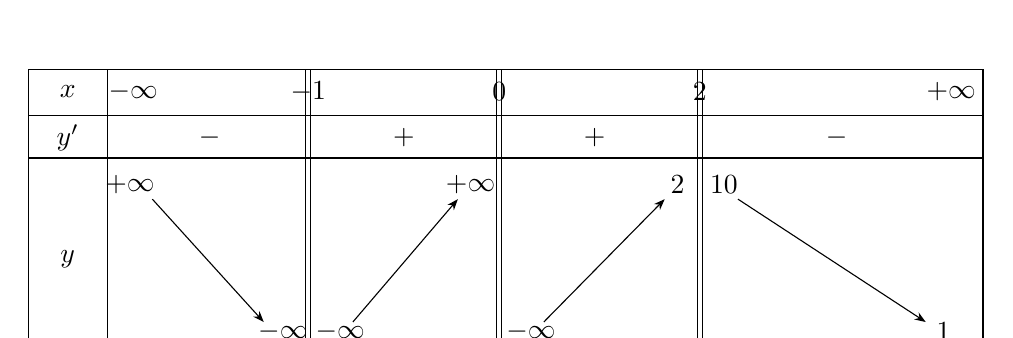
\begin{tikzpicture}[x=\dimexpr\linewidth/15\relax,y=-0.83cm,
  every node/.style={font=\fontsize{10}{12}\selectfont}]
  \draw[thin] (0,0) rectangle (15,4.3);
  \draw[thin] (1.25,0) -- (1.25,4.3);
  \draw[thin] (0,0.7) -- (15,0.7);
  \draw[thin] (0,1.35) -- (15,1.35);
  \foreach \xx in {4.4,7.4,10.55}{
    \draw[thin] (\xx-0.04,0) -- (\xx-0.04,4.3);
    \draw[thin] (\xx+0.04,0) -- (\xx+0.04,4.3);
  }
  \node at (0.62,0.34) {$x$};
  \node at (0.62,1.04) {$y'$};
  \node at (0.62,2.9) {$y$};
  \node at (1.65,0.34) {$-\infty$};
  \node at (4.4,0.34) {$-1$};
  \node at (7.4,0.34) {$0$};
  \node at (10.55,0.34) {$2$};
  \node at (14.5,0.34) {$+\infty$};
  \node at (2.85,1.04) {$-$};
  \node at (5.9,1.04) {$+$};
  \node at (8.9,1.04) {$+$};
  \node at (12.7,1.04) {$-$};
  \node at (1.6,1.75) {$+\infty$};
  \node at (4.0,4.0) {$-\infty$};
  \node at (4.9,4.0) {$-\infty$};
  \node at (6.95,1.75) {$+\infty$};
  \node at (7.9,4.0) {$-\infty$};
  \node at (10.2,1.75) {$2$};
  \node at (10.93,1.75) {$10$};
  \node at (14.38,4.0) {$1$};
  \draw[thin,-{Stealth[length=4pt]}] (1.95,1.98) -- (3.7,3.86);
  \draw[thin,-{Stealth[length=4pt]}] (5.1,3.86) -- (6.75,1.98);
  \draw[thin,-{Stealth[length=4pt]}] (8.1,3.86) -- (10.0,1.98);
  \draw[thin,-{Stealth[length=4pt]}] (11.15,1.98) -- (14.1,3.86);
\end{tikzpicture}
\end{notebox}%
}


% Đồ thị câu 15: một nghiệm âm, cực tiểu dương phía trên trục Ox.
\newcommand{\graphfifteen}{%
\begin{notebox}
\centering
\begin{tikzpicture}[x=0.70cm,y=0.60cm,
 every node/.style={font=\fontsize{11}{13}\selectfont}]
 \draw[thin,-{Stealth[length=4pt]}] (-5.4,0) -- (5.5,0) node[below] {$x$};
 \draw[thin,-{Stealth[length=4pt]}] (0,-1.8) -- (0,4.35) node[right] {$y$};
 \draw[sectionpurple,thick]
   (-4.0,-1.40) .. controls (-2.7,0.5) and (-1.25,2.45) .. (0.75,3.0)
   .. controls (1.65,3.12) and (2.45,0.40) .. (3.05,0.38)
   .. controls (3.7,0.37) and (4.12,2.10) .. (4.45,4.1);
 \fill (0,0) circle (1.4pt);
 \node[below left] at (0,0) {$O$};
\end{tikzpicture}
\end{notebox}%
}
% Bảng biến thiên câu 19.
\newcommand{\bbtnineteen}{%
\begin{notebox}
\centering
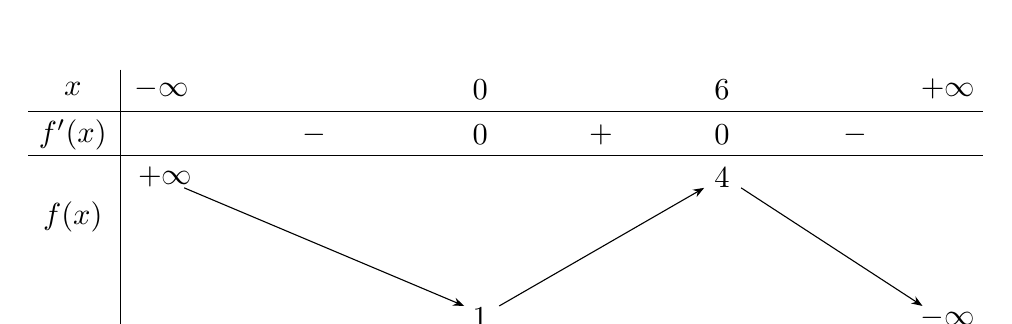
\begin{tikzpicture}[x=\dimexpr\linewidth/15\relax,y=-0.75cm,
 every node/.style={font=\fontsize{11}{13}\selectfont}]
 \draw[thin] (0,0.7) -- (15,0.7);
 \draw[thin] (0,1.45) -- (15,1.45);
 \draw[thin] (1.45,0) -- (1.45,4.5);
 \node at (0.7,0.33) {$x$};
 \node at (0.7,1.1) {$f'(x)$};
 \node at (0.7,2.5) {$f(x)$};
 \node at (2.1,0.33) {$-\infty$};
 \node at (7.1,0.33) {$0$};
 \node at (10.9,0.33) {$6$};
 \node at (14.45,0.33) {$+\infty$};
 \node at (4.5,1.1) {$-$};
 \node at (7.1,1.1) {$0$};
 \node at (9.0,1.1) {$+$};
 \node at (10.9,1.1) {$0$};
 \node at (13.0,1.1) {$-$};
 \node at (2.15,1.82) {$+\infty$};
 \node at (7.1,4.2) {$1$};
 \node at (10.9,1.82) {$4$};
 \node at (14.45,4.2) {$-\infty$};
 \draw[thin,-{Stealth[length=4pt]}] (2.45,2.0) -- (6.85,4.0);
 \draw[thin,-{Stealth[length=4pt]}] (7.4,4.0) -- (10.62,2.0);
 \draw[thin,-{Stealth[length=4pt]}] (11.2,2.0) -- (14.05,4.0);
\end{tikzpicture}
\end{notebox}%
}


\begin{document}
\fontsize{12}{15}\selectfont

{\centering
\textbf{ĐỀ TDMXX08}\par
\textbf{CƠ BẢN VỀ TIỆM CẬN ĐỨNG VÀ TIỆM CẬN NGANG CỦA ĐỒ THỊ HÀM SỐ}\par
{\fontsize{10.5}{13}\selectfont\itshape
Form đề chuẩn bám sát BGD2026 -- Thời gian làm bài \textbf{90 phút}\par}}

\textbf{Phần I. Câu trắc nghiệm nhiều phương án lựa chọn.}
Thí sinh trả lời từ câu 1 đến câu 12. Mỗi câu hỏi thí sinh chỉ chọn một phương án.

\question[TDM21]{1} TCN của đồ thị của hàm số $y=\dfrac{2x-1}{x+1}$ là
\fourchoices{$y=-2$}{$y=2$}{$y=1$}{$x=-1$}

\question[TDM21]{2} TCĐ của đồ thị của hàm số $y=\dfrac{3x+1}{x-2}$ là
\fourchoices{$y=2$}{$y=3$}{$x=2$}{$x=-\dfrac{1}{3}$}

\question[TDM21]{3} Đồ thị của hàm số $y=\dfrac{\sqrt{2x^{2}-1}}{x^{2}+2x+5}$ có số đường tiệm cận ngang là
\fourchoices{$1$}{$0$}{$2$}{$3$}

\question[TDM21]{4} Đồ thị của hàm số $y=\dfrac{|x+1|}{2x+5}$ có số đường tiệm cận ngang là
\fourchoices{$1$}{$2$}{$3$}{$0$}

\question[TDM21]{5} Đồ thị của hàm số $y=\dfrac{\sqrt{2x^{6}-1}}{x^{2}+2x+5}$ có số đường tiệm cận ngang là
\fourchoices{$1$}{$0$}{$2$}{$3$}

\question[TDM21]{6} Đồ thị của hàm số $y=\dfrac{|x+2|}{x-1}$ có số đường tiệm cận là
\fourchoices{$1$}{$3$}{$2$}{$0$}

\question[TDM21]{7} Cho hàm số $y=f(x)$ có bảng biến thiên như hình vẽ bên dưới.
Hãy chọn kết luận \textbf{đúng} về tiệm cận đứng và tiệm cận ngang của đồ thị hàm số $y=f(x)$?
\bbtseven
\par\noindent\answerlabel{A} Đồ thị hàm số có hai TCĐ là $x=-1$; $x=0$ và một TCN là $y=1$.\par
\noindent\answerlabel{B} Đồ thị hàm số có ba TCĐ là $x=-1$; $x=0$; $x=2$ và một TCN là $y=1$.\par
\noindent\answerlabel{C} Đồ thị hàm số có $3$ TCĐ và $2$ TCN.\par
\noindent\answerlabel{D} Đồ thị hàm số không có TCN và có $2$ TCĐ.\par
\newpage



\question[TDM31]{8} Đồ thị của hàm số $y=\dfrac{\sqrt{1-x^{2}}}{x^{2}-4}$ có số đường tiệm cận là
\fourchoices{$1$}{$2$}{$3$}{$0$}

\question[TDM31]{9} Số đường tiệm cận của đồ thị hàm số
$y=\dfrac{\sqrt{x^{2}-4}+x^{2}-2}{3x^{2}-10x+3}$ là
\fourchoices{$2$}{$0$}{$1$}{$3$}

\question[TDM32]{10} Số đường tiệm cận đứng và tiệm cận ngang của đồ thị hàm số
$y=\dfrac{x+1}{|x|+1}$ là
\fourchoices{$2$}{$3$}{$1$}{$0$}

\question[TDM31]{11} Cho hàm số $y=f(x)$ có tập xác định $\mathbb{R}$ và có đồ thị $(C)$.
Biết các giới hạn
$\displaystyle\lim_{x\to+\infty}f(x)=m^{2}-5m$,
$\displaystyle\lim_{x\to-\infty}f(x)=m-5$.
Hỏi có tất cả bao nhiêu tham số $m$ để đồ thị $(C)$ có đúng một đường tiệm cận ngang?
\fourchoices{$2$}{$1$}{$0$}{$3$}

\question[TDM32]{12} Cho hàm số $y=\dfrac{mx+2}{2x-m+3}$ có đồ thị $(C)$.
Gọi $S$ là tập chứa tất cả các giá trị thực của tham số $m$ để tiệm cận của đồ thị $(C)$
đi qua điểm $A(3;2)$. Tổng tất cả các phần tử của tập $S$ bằng:
\fourchoices{$9$}{$22$}{$13$}{$2$}

\par\addvspace{7pt}
\textbf{Phần II. Câu trắc nghiệm đúng sai.}
Thí sinh trả lời từ câu 13 đến câu 16. Trong mỗi ý \textbf{a), b), c), d)} ở mỗi câu,
thí sinh chọn \textbf{đúng} hoặc \textbf{sai}.

\question[TDM22]{13} Cho hàm số $y=f(x)$ có đồ thị $(C)$.
Hỏi trong các mệnh đề dưới đây, mệnh đề nào \textbf{đúng}, mệnh đề nào \textbf{sai}?
\tfbox
{Tiệm cận ngang của $(C)$ có thể cắt $(C)$.}
{Tiệm cận ngang của $(C)$ không thể có điểm chung với $(C)$.}
{Đồ thị $(C)$ có tối đa hai tiệm cận ngang.}
{Đồ thị $(C)$ luôn có ít nhất một tiệm cận ngang.}

\question[TDM22]{14} Cho hàm số $y=f(x)$ có đồ thị $(C)$.
Hỏi trong các mệnh đề dưới đây, mệnh đề nào \textbf{đúng}, mệnh đề nào \textbf{sai}?
\tfbox
{Đồ thị $(C)$ có thể cắt đường tiệm cận ngang của nó.}
{Đồ thị $(C)$ và đường tiệm đứng của nó có thể có điểm chung.}
{Đồ thị $(C)$ có thể có vô số các đường tiệm cận đứng.}
{Đồ thị $(C)$ có tối thiểu một đường tiệm cận đứng.}

\newpage



\question[TDM32]{15} Cho hàm số $y=f(x)$ có đồ thị như hình vẽ. Gọi $(C)$ là đồ thị của hàm số
$y=\dfrac{1}{f(x)}$.
\graphfifteen
Hỏi trong các mệnh đề dưới đây, mệnh đề nào \textbf{đúng}, mệnh đề nào \textbf{sai}?
\tfbox
{Đồ thị $(C)$ có hai đường tiệm cận ngang.}
{Đường thẳng $y=0$ là một tiệm cận ngang của $(C)$.}
{Đồ thị $(C)$ có đúng một đường tiệm cận đứng.}
{Đồ thị $(C)$ có tất cả $3$ đường tiệm cận đứng và ngang.}

\question[TDM32]{16} Cho hàm số $y=\dfrac{x^{2}-2(a-1)x+a+3}{x^{2}-3x-4}$ có đồ thị $(C)$,
với $a$ là số thực.
Hỏi trong các mệnh đề dưới đây, mệnh đề nào \textbf{đúng}, mệnh đề nào \textbf{sai}?
\tfbox
{Đồ thị $(C)$ có đúng một đường tiệm cận ngang $y=0$.}
{Khi $a=-\dfrac{2}{3}$ thì $(C)$ có đúng một đường tiệm cận.}
{Khi $a=\dfrac{27}{7}$ thì $(C)$ có đúng hai đường tiệm cận.}
{Tổng tất cả các giá trị của $a$ để $(C)$ có hai đường tiệm cận là $\dfrac{67}{21}$.}

\par\addvspace{7pt}
\textbf{Phần III. Câu trắc nghiệm trả lời ngắn.}
Thí sinh trả lời từ câu 17 đến câu 22.

\question[TDM31]{17} Cho hàm số
$y=\dfrac{\sqrt{x^{2}-4x+3}-2}{x-2}$ có đồ thị $(C)$.
Số tiệm cận của đồ thị $(C)$ là
\shortanswer

\question[TDM31]{18} Tổng số tiệm cận của đồ thị hàm số
$y=\dfrac{\sqrt{5-x^{2}}-x-1}{x^{2}+5x-6}$ bằng bao nhiêu?
\shortanswer

\newpage



\question[TDM32]{19} Cho hàm bậc ba $y=f(x)$ có bảng biến thiên như hình vẽ bên dưới.
\bbtnineteen
Số đường tiệm cận đứng của đồ thị hàm số
$y=\dfrac{\sqrt{x^{2}+1}-1}{f(x)-1}$ là?
\shortanswer

\question[TDM32]{20} Biết đồ thị hàm số
$y=\dfrac{(4a-b)x^{2}+ax+1}{x^{2}+ax+b-12}$
nhận trục hoành và trục tung làm hai tiệm cận.
Hãy tính giá trị của biểu thức $(a+b)$?
\shortanswer

\question[TDM32]{21} Gọi $S$ là tập chứa tất cả các giá trị thực của $a$ để đồ thị hàm số
$y=\dfrac{x^{2}-(2a-1)x+a}{x^{3}-3x^{2}+2x}$
có đúng ba đường tiệm cận. Số phần tử của tập $S$ là:
\shortanswer

\question[TDM32]{22} Biết rằng đồ thị của hàm số
$y=\dfrac{\sqrt{x+5}+ax+b}{(x+1)^{2}}$
không có tiệm cận đứng. Khi đó tổng $(a^{2}+b^{2})$ bằng bao nhiêu
(làm tròn kết quả đến hàng phần mười)?
\shortanswer

\par\medskip
{\centering\textbf{\textcolor{sectionpurple}{--- Hết ---}}\par}

% Nguồn nội dung: Đề TDMXX08, Nguyễn Đăng Ái -- Tài liệu Ôn Thi .NET.
% Bản LaTeX được biên tập theo phong cách BTVN_01_B1.tex.
\end{document}
